\documentclass{standalone}
\usepackage{tikz}
\usetikzlibrary{patterns, positioning}

\begin{document}
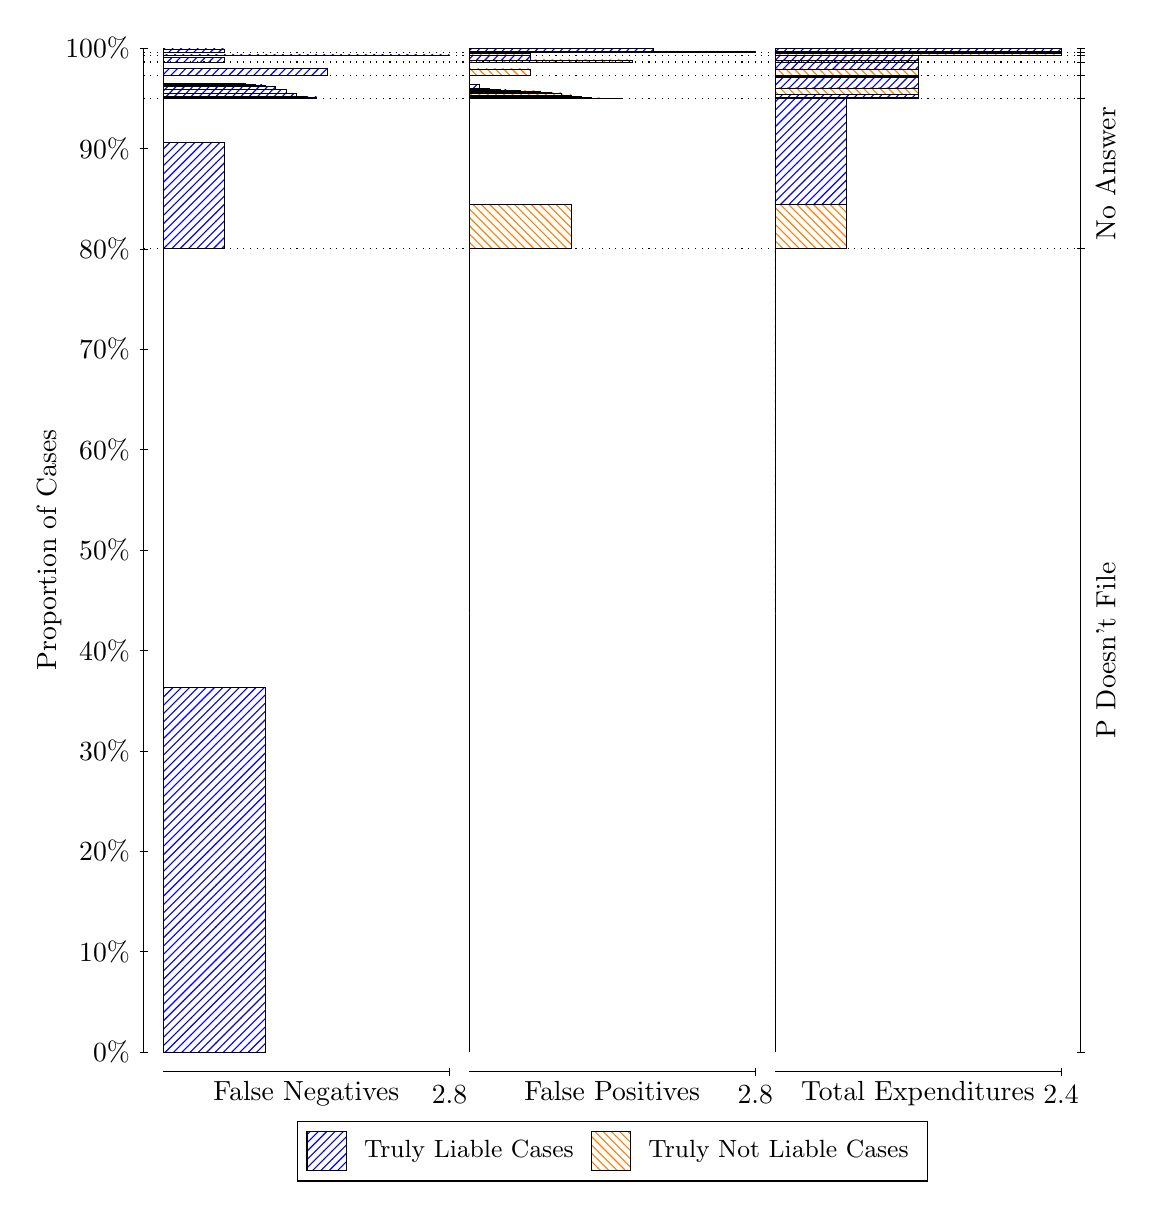
\begin{tikzpicture}
\draw[black, very thin] (1.5,1.75) -- (1.5,14.5);
\node[rotate=90, anchor=center] at (0.3, 8.125) {Proportion of Cases};
\draw[black, very thin] (1.45,1.75) -- (1.55,1.75);
\node[anchor=east] at (1.45, 1.75) {0\%};
\draw[black, very thin] (1.45,3.025) -- (1.55,3.025);
\node[anchor=east] at (1.45, 3.025) {10\%};
\draw[black, very thin] (1.45,4.3) -- (1.55,4.3);
\node[anchor=east] at (1.45, 4.3) {20\%};
\draw[black, very thin] (1.45,5.575) -- (1.55,5.575);
\node[anchor=east] at (1.45, 5.575) {30\%};
\draw[black, very thin] (1.45,6.85) -- (1.55,6.85);
\node[anchor=east] at (1.45, 6.85) {40\%};
\draw[black, very thin] (1.45,8.125) -- (1.55,8.125);
\node[anchor=east] at (1.45, 8.125) {50\%};
\draw[black, very thin] (1.45,9.4) -- (1.55,9.4);
\node[anchor=east] at (1.45, 9.4) {60\%};
\draw[black, very thin] (1.45,10.675) -- (1.55,10.675);
\node[anchor=east] at (1.45, 10.675) {70\%};
\draw[black, very thin] (1.45,11.95) -- (1.55,11.95);
\node[anchor=east] at (1.45, 11.95) {80\%};
\draw[black, very thin] (1.45,13.225) -- (1.55,13.225);
\node[anchor=east] at (1.45, 13.225) {90\%};
\draw[black, very thin] (1.45,14.5) -- (1.55,14.5);
\node[anchor=east] at (1.45, 14.5) {100\%};

\draw[black, very thin] (13.4,1.75) -- (13.4,14.5);
\draw[black, very thin] (13.35,1.75) -- (13.45,1.75);
\node[anchor=west] at (13.35, 1.75) {};
\draw[black, very thin] (13.35,11.955) -- (13.45,11.955);
\node[anchor=west] at (13.35, 11.955) {};
\draw[black, very thin] (13.35,13.857) -- (13.45,13.857);
\node[anchor=west] at (13.35, 13.857) {};
\draw[black, very thin] (13.35,14.152) -- (13.45,14.152);
\node[anchor=west] at (13.35, 14.152) {};
\draw[black, very thin] (13.35,14.323) -- (13.45,14.323);
\node[anchor=west] at (13.35, 14.323) {};
\draw[black, very thin] (13.35,14.404) -- (13.45,14.404);
\node[anchor=west] at (13.35, 14.404) {};
\draw[black, very thin] (13.35,14.444) -- (13.45,14.444);
\node[anchor=west] at (13.35, 14.444) {};
\draw[black, very thin] (13.35,14.5) -- (13.45,14.5);
\node[anchor=west] at (13.35, 14.5) {};

\draw[black, very thin, pattern color=blue, pattern=north east lines] (1.75,1.75) rectangle (3.0476,6.3838);
\draw[black, very thin, pattern color=orange, pattern=north west lines] (1.75,6.3838) rectangle (1.75,11.955);
\draw[black, very thin, pattern color=blue, pattern=north east lines] (1.75,11.955) rectangle (2.5286,13.302);
\draw[black, very thin, pattern color=orange, pattern=north west lines] (1.75,13.302) rectangle (1.75,13.857);
\draw[black, very thin, pattern color=blue, pattern=north east lines] (1.75,13.857) rectangle (3.6964,13.879);
\draw[black, very thin, pattern color=blue, pattern=north east lines] (1.75,13.879) rectangle (3.5667,13.885);
\draw[black, very thin, pattern color=blue, pattern=north east lines] (1.75,13.885) rectangle (3.4369,13.921);
\draw[black, very thin, pattern color=blue, pattern=north east lines] (1.75,13.921) rectangle (3.3071,13.974);
\draw[black, very thin, pattern color=blue, pattern=north east lines] (1.75,13.974) rectangle (3.1774,14.017);
\draw[black, very thin, pattern color=blue, pattern=north east lines] (1.75,14.017) rectangle (3.0476,14.032);
\draw[black, very thin, pattern color=blue, pattern=north east lines] (1.75,14.032) rectangle (2.9179,14.042);
\draw[black, very thin, pattern color=blue, pattern=north east lines] (1.75,14.042) rectangle (2.7881,14.048);
\draw[black, very thin, pattern color=blue, pattern=north east lines] (1.75,14.048) rectangle (2.6583,14.052);
\draw[black, very thin, pattern color=orange, pattern=north west lines] (1.75,14.052) rectangle (1.75,14.152);
\draw[black, very thin, pattern color=blue, pattern=north east lines] (1.75,14.152) rectangle (3.8262,14.24);
\draw[black, very thin, pattern color=orange, pattern=north west lines] (1.75,14.24) rectangle (1.75,14.323);
\draw[black, very thin, pattern color=blue, pattern=north east lines] (1.75,14.323) rectangle (2.5286,14.378);
\draw[black, very thin, pattern color=orange, pattern=north west lines] (1.75,14.378) rectangle (1.75,14.404);
\draw[black, very thin, pattern color=blue, pattern=north east lines] (1.75,14.404) rectangle (5.3833,14.414);
\draw[black, very thin, pattern color=orange, pattern=north west lines] (1.75,14.414) rectangle (1.75,14.444);
\draw[black, very thin, pattern color=blue, pattern=north east lines] (1.75,14.444) rectangle (2.5286,14.49);
\draw[black, very thin, pattern color=orange, pattern=north west lines] (1.75,14.49) rectangle (1.75,14.5);
\draw[black, very thin, pattern color=orange, pattern=north west lines] (5.6333,1.75) rectangle (5.6333,7.3207);
\draw[black, very thin, pattern color=blue, pattern=north east lines] (5.6333,7.3207) rectangle (5.6333,11.955);
\draw[black, very thin, pattern color=orange, pattern=north west lines] (5.6333,11.955) rectangle (6.931,12.51);
\draw[black, very thin, pattern color=blue, pattern=north east lines] (5.6333,12.51) rectangle (5.6333,13.857);
\draw[black, very thin, pattern color=orange, pattern=north west lines] (5.6333,13.857) rectangle (7.5798,13.859);
\draw[black, very thin, pattern color=orange, pattern=north west lines] (5.6333,13.859) rectangle (7.45,13.862);
\draw[black, very thin, pattern color=orange, pattern=north west lines] (5.6333,13.862) rectangle (7.3202,13.866);
\draw[black, very thin, pattern color=orange, pattern=north west lines] (5.6333,13.866) rectangle (7.1905,13.874);
\draw[black, very thin, pattern color=orange, pattern=north west lines] (5.6333,13.874) rectangle (7.0607,13.888);
\draw[black, very thin, pattern color=orange, pattern=north west lines] (5.6333,13.888) rectangle (6.931,13.906);
\draw[black, very thin, pattern color=orange, pattern=north west lines] (5.6333,13.906) rectangle (6.8012,13.929);
\draw[black, very thin, pattern color=orange, pattern=north west lines] (5.6333,13.929) rectangle (6.6714,13.937);
\draw[black, very thin, pattern color=orange, pattern=north west lines] (5.6333,13.937) rectangle (6.5417,13.957);
\draw[black, very thin, pattern color=blue, pattern=north east lines] (5.6333,13.957) rectangle (6.2821,13.961);
\draw[black, very thin, pattern color=blue, pattern=north east lines] (5.6333,13.961) rectangle (6.1524,13.967);
\draw[black, very thin, pattern color=blue, pattern=north east lines] (5.6333,13.967) rectangle (6.0226,13.977);
\draw[black, very thin, pattern color=blue, pattern=north east lines] (5.6333,13.977) rectangle (5.8929,13.992);
\draw[black, very thin, pattern color=blue, pattern=north east lines] (5.6333,13.992) rectangle (5.7631,14.035);
\draw[black, very thin, pattern color=blue, pattern=north east lines] (5.6333,14.035) rectangle (5.6333,14.152);
\draw[black, very thin, pattern color=orange, pattern=north west lines] (5.6333,14.152) rectangle (6.4119,14.236);
\draw[black, very thin, pattern color=blue, pattern=north east lines] (5.6333,14.236) rectangle (5.6333,14.323);
\draw[black, very thin, pattern color=orange, pattern=north west lines] (5.6333,14.323) rectangle (7.7095,14.349);
\draw[black, very thin, pattern color=blue, pattern=north east lines] (5.6333,14.349) rectangle (6.4119,14.404);
\draw[black, very thin, pattern color=orange, pattern=north west lines] (5.6333,14.404) rectangle (6.4119,14.434);
\draw[black, very thin, pattern color=blue, pattern=north east lines] (5.6333,14.434) rectangle (5.6333,14.444);
\draw[black, very thin, pattern color=orange, pattern=north west lines] (5.6333,14.444) rectangle (9.2667,14.454);
\draw[black, very thin, pattern color=blue, pattern=north east lines] (5.6333,14.454) rectangle (7.969,14.5);
\draw[black, very thin, pattern color=orange, pattern=north west lines] (9.5167,1.75) rectangle (9.5167,7.3207);
\draw[black, very thin, pattern color=blue, pattern=north east lines] (9.5167,7.3207) rectangle (9.5167,11.955);
\draw[black, very thin, pattern color=orange, pattern=north west lines] (9.5167,11.955) rectangle (10.425,12.51);
\draw[black, very thin, pattern color=blue, pattern=north east lines] (9.5167,12.51) rectangle (10.425,13.857);
\draw[black, very thin, pattern color=orange, pattern=north west lines] (9.5167,13.857) rectangle (11.333,13.872);
\draw[black, very thin, pattern color=blue, pattern=north east lines] (9.5167,13.872) rectangle (11.333,13.915);
\draw[black, very thin, pattern color=orange, pattern=north west lines] (9.5167,13.915) rectangle (11.333,13.993);
\draw[black, very thin, pattern color=blue, pattern=north east lines] (9.5167,13.993) rectangle (11.333,14.129);
\draw[black, very thin, pattern color=orange, pattern=north west lines] (9.5167,14.129) rectangle (11.333,14.136);
\draw[black, very thin, pattern color=blue, pattern=north east lines] (9.5167,14.136) rectangle (11.333,14.152);
\draw[black, very thin, pattern color=orange, pattern=north west lines] (9.5167,14.152) rectangle (11.333,14.236);
\draw[black, very thin, pattern color=blue, pattern=north east lines] (9.5167,14.236) rectangle (11.333,14.323);
\draw[black, very thin, pattern color=orange, pattern=north west lines] (9.5167,14.323) rectangle (11.333,14.349);
\draw[black, very thin, pattern color=blue, pattern=north east lines] (9.5167,14.349) rectangle (11.333,14.404);
\draw[black, very thin, pattern color=orange, pattern=north west lines] (9.5167,14.404) rectangle (13.15,14.434);
\draw[black, very thin, pattern color=blue, pattern=north east lines] (9.5167,14.434) rectangle (13.15,14.444);
\draw[black, very thin, pattern color=orange, pattern=north west lines] (9.5167,14.444) rectangle (13.15,14.454);
\draw[black, very thin, pattern color=blue, pattern=north east lines] (9.5167,14.454) rectangle (13.15,14.5);
\draw[black, dotted] (1.5,11.955) -- (13.4,11.955);
\draw[black, dotted] (1.5,13.857) -- (13.4,13.857);
\draw[black, dotted] (1.5,14.152) -- (13.4,14.152);
\draw[black, dotted] (1.5,14.323) -- (13.4,14.323);
\draw[black, dotted] (1.5,14.404) -- (13.4,14.404);
\draw[black, dotted] (1.5,14.444) -- (13.4,14.444);
\draw[black, very thin] (1.75,1.5) -- (5.3833,1.5);
\node[anchor=north] at (3.5667, 1.5) {False Negatives};
\draw[black, very thin] (5.3833,1.45) -- (5.3833,1.55);
\node[anchor=north] at (5.3833, 1.45) {2.8};

\draw[black, very thin] (5.6333,1.5) -- (9.2667,1.5);
\node[anchor=north] at (7.45, 1.5) {False Positives};
\draw[black, very thin] (9.2667,1.45) -- (9.2667,1.55);
\node[anchor=north] at (9.2667, 1.45) {2.8};

\draw[black, very thin] (9.5167,1.5) -- (13.15,1.5);
\node[anchor=north] at (11.333, 1.5) {Total Expenditures};
\draw[black, very thin] (13.15,1.45) -- (13.15,1.55);
\node[anchor=north] at (13.15, 1.45) {2.4};

\node[black, centered, rotate=90] at (13.72, 6.8523) {P Doesn't File};
\node[black, centered, rotate=90] at (13.72, 12.906) {No Answer};






\draw (7.449999999999999,1.5) node[draw=none] (baseCoordinate) {};
\begin{scope}[align=center]
        \matrix[scale=0.5, draw=black, below=0.5cm of baseCoordinate, nodes={draw}, column sep=0.1cm]{
            \node[rectangle, draw, minimum width=0.5cm, minimum height=0.5cm, pattern=north east lines, pattern color=blue] {}; &
            \node[draw=none, font=\small] (B) {Truly Liable Cases}; &
            \node[rectangle, draw, minimum width=0.5cm, minimum height=0.5cm, pattern=north west lines, pattern color=orange] {}; &
            \node[draw=none, font=\small] (B) {Truly Not Liable Cases}; \\
            };
\end{scope}

\end{tikzpicture}
\end{document}